\documentclass{article}

% if you need to pass options to natbib, use, e.g.:
% \PassOptionsToPackage{numbers, compress}{natbib}
% before loading nips_2016
%
% to avoid loading the natbib package, add option nonatbib:
% \usepackage[nonatbib]{nips_2016}

% \usepackage{nips_2016}

% to compile a camera-ready version, add the [final] option, e.g.:
\usepackage[final]{10707hw1_template}

\usepackage[utf8]{inputenc} % allow utf-8 input
\usepackage[T1]{fontenc}    % use 8-bit T1 fonts
\usepackage{hyperref}       % hyperlinks
\usepackage{url}            % simple URL typesetting
\usepackage{booktabs}       % professional-quality tables
\usepackage{amsfonts}       % blackboard math symbols
\usepackage{nicefrac}       % compact symbols for 1/2, etc.
\usepackage{microtype}      % microtypography
\usepackage{amsmath}
\usepackage{caption}
\usepackage{subcaption}
\usepackage{graphicx}

\title{10707 Homework 1}

% The \author macro works with any number of authors. There are two
% commands used to separate the names and addresses of multiple
% authors: \And and \AND.
%
% Using \And between authors leaves it to LaTeX to determine where to
% break the lines. Using \AND forces a line break at that point. So,
% if LaTeX puts 3 of 4 authors names on the first line, and the last
% on the second line, try using \AND instead of \And before the third
% author name.

\author{
  David S.~Hippocampus\thanks{Use footnote for providing further
    information about author (webpage, alternative
    address)---\emph{not} for acknowledging funding agencies.} \\
  Department of Computer Science\\
  Cranberry-Lemon University\\
  Pittsburgh, PA 15213 \\
  \texttt{hippo@cs.cranberry-lemon.edu} \\
  %% examples of more authors
  %% \And
  %% Coauthor \\
  %% Affiliation \\
  %% Address \\
  %% \texttt{email} \\
  %% \AND
  %% Coauthor \\
  %% Affiliation \\
  %% Address \\
  %% \texttt{email} \\
  %% \And
  %% Coauthor \\
  %% Affiliation \\
  %% Address \\
  %% \texttt{email} \\
  %% \And
  %% Coauthor \\
  %% Affiliation \\
  %% Address \\
  %% \texttt{email} \\
}

\begin{document}
% \nipsfinalcopy is no longer used

\maketitle


\section*{Problem 1 (6 pts)}
This question will test your general understanding of overfitting 
as they relate to model complexity and training set size. 
Consider a continuous domain and a smooth joint distribution over 
inputs and outputs, so that no test or training case is ever duplicated exactly.
\begin{itemize}
\item 
For a fixed training set size, sketch a graph of the typical 
behavior of training error rate (y-axis) versus model complexity (x-axis).
Add to this graph a curve showing the typical behavior of the corresponding test 
error rate versus model complexity, on the same axes. (Assume that we have an infinite test set drawn independently from the 
same joint distribution as the training set).
Mark a vertical line showing where you think the most complex model 
your data supports is; chose your horizontal range so that this line is 
neither on the extreme left nor on the extreme right. Indicate on your vertical 
axes where zero error is and draw your graphs with increasing error upwards and 
increasing complexity rightwards. \\

\item  For a fixed model complexity, sketch a graph of the typical 
behavior of training error rate (y-axis) versus training set size (x-axis). 
Add to this graph a curve showing the typical behavior of test error rate 
versus training set size, on the same axes
(again on an iid infinite test set). 
Indicate on your vertical axes where zero error is and draw your graphs with increasing error 
upwards and increasing training set size rightwards. \\

\item One of the commonly used regularization methods in neural networks is \emph{early stopping}. Argue qualitatively why (or why not) early stopping is a reasonable regularization metric. 

\end{itemize} 


\subsection*{Your answer here}

1. Graph shown in Figure ~\ref{fig:1a}.

\begin{figure}[h]
\centering
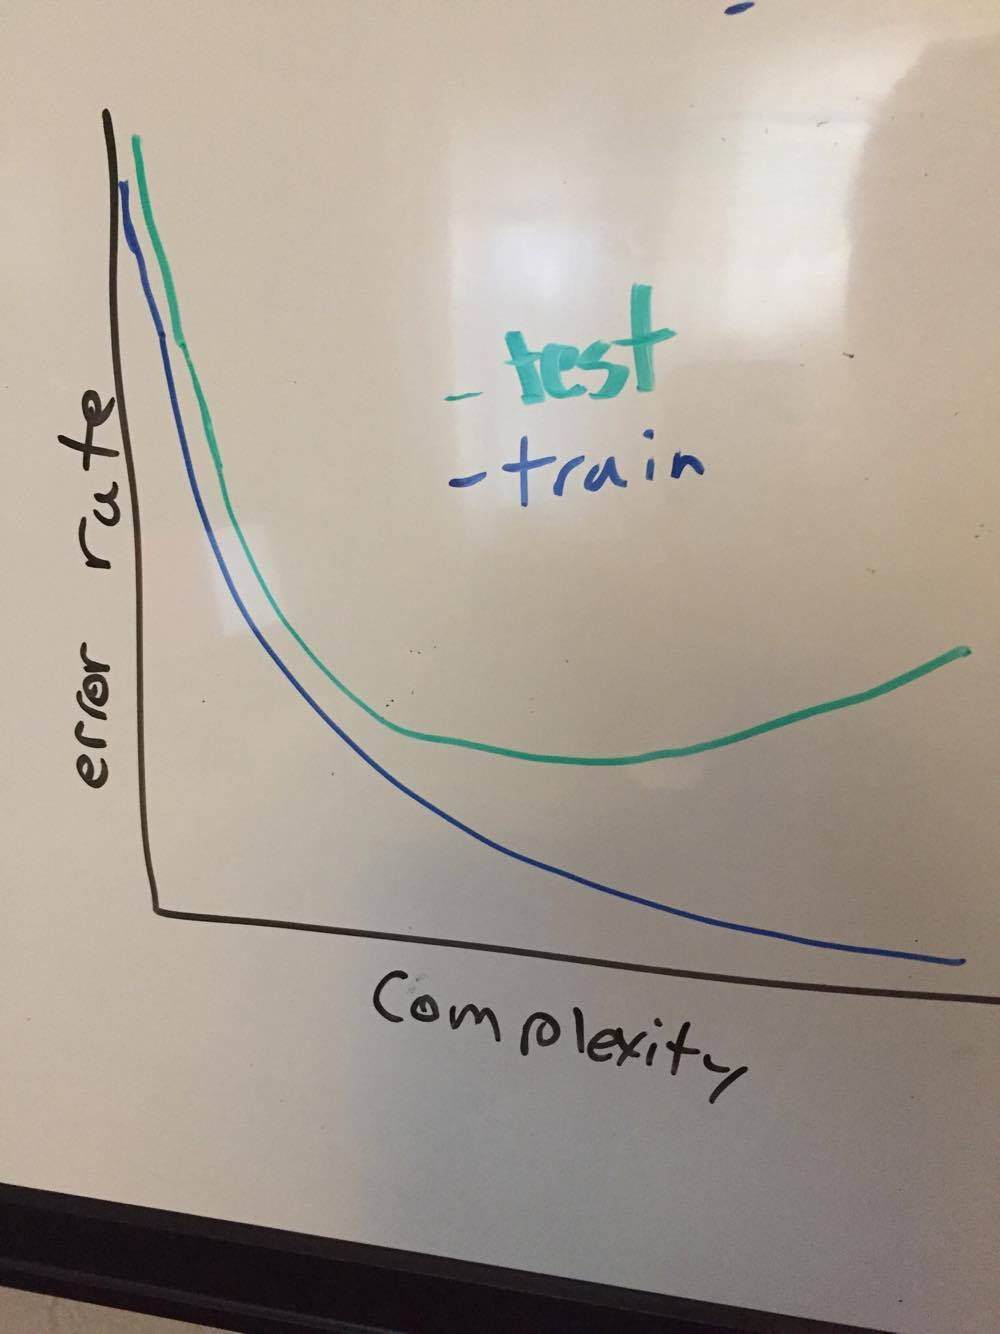
\includegraphics[width=.3\linewidth]{1a.jpg}
\caption{error rate vs complexity}
\label{fig:1a}
\end{figure}



2. Graph shown in Figure ~\ref{fig:1b}.

\begin{figure}[h]
\centering
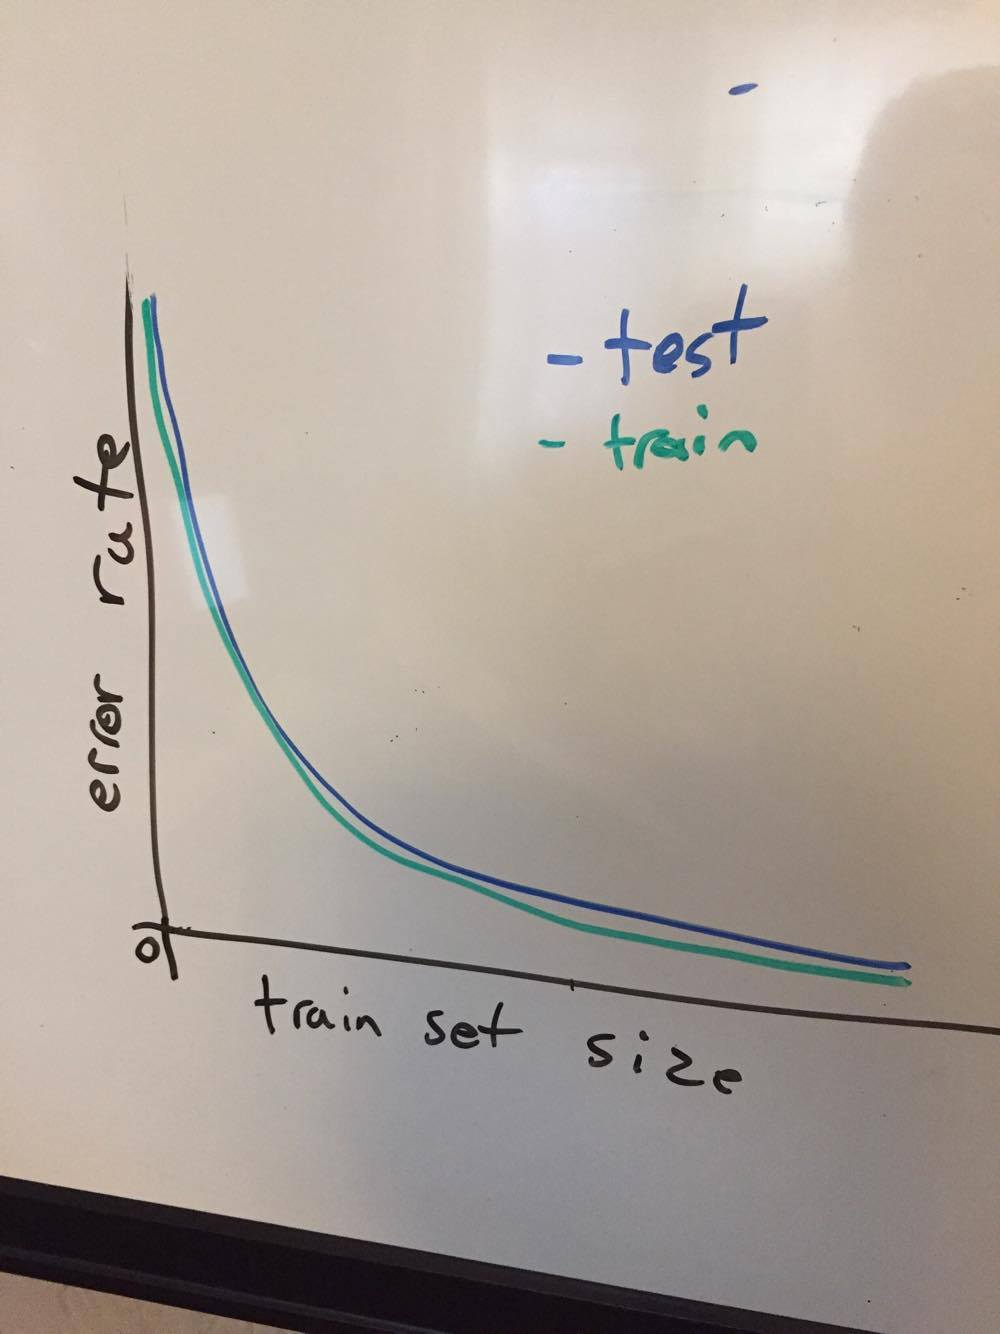
\includegraphics[width=.3\linewidth]{1b.jpg}
\caption{error rate vs dataset size}
\label{fig:1b}
\end{figure}

3. Yes, it is a reasonable regularization metric. As a network trains more and more, the weights tune directly to the data in the training set. The problem with this is that the network may begin to start looking at specific noise in the training set that may not be represented in the test set. The more the network trains, the more the weights are specifically tuned to the training set, and at some point it will likely be tuned to where it is overfit. Stopping early prevents the network from training to the point where it knows every detail of the test set, which can improve generalization. T



testingtesting
%\section*{Problem 2 (12 pts)}
%In this question we will study the expected loss for regression problems.
%Consider the expected $L_q$ loss function given by:
%\beqa
%\mathbb{E}[L_q] = \iint | y(\bx) - t | ^q p(\bx,t) \d t \d\bx
%\eeqa
%Show that:
%\begin{enumerate}
%\item[a)] The minimum expected loss for $q=1$
%is given by the conditional median (i.e. by the
%function $y(\bx)$ such that the probability mass for $t < y(\bx)$
%is the same as for $t \geq y(\bx)$).
%\item[b)] The minimum expected loss for $q \rightarrow 0$
%is given by the conditional mode (i.e. by the function $y(\bx)$
%equal to the value of $t$ that maximizes $p(t | \bx)$ for each $\bx$).
%\end{enumerate}


\section*{Problem 2 (8 pts)}

Consider $N$ training points $(x_i, y_i)$ drawn i.i.d from a distribution that is characterized as: 
\begin{align}
x_i &\sim h(x) \\
y_i &= f(x_i) + \epsilon_i \\
\epsilon_i &\sim (0, \sigma^2) 
\end{align}

where $f$ is the regression function. An estimator for this data, \emph{linear} in $y_i$ is given by

\begin{equation}
    \hat f(x^*) = \sum_{i=1}^{N} l_i(x^* ; \mathcal{X})y_i, 
\end{equation}

where $l_i(x^*; \mathcal{X})$ depends on the entire training sequence of $x_i$ (denoted by $\mathcal{X}$)  but do not depend on $y_i$. Show that k-nearest-neighbor regression and linear regression are members of this class of estimators. What would be the $l_i(x^* ; \mathcal{X})$ in both these regressions (knn and linear)? 


\subsection*{Your answer here}

%\section*{Problem 3 (6 pts)}
%Consider the binary-class problem, show that for a linearly separable dataset, the maximum likelihood solution
%for a logistic regression model is obtained by finding a vector $\bw$
%whose decision boundary $\bw^{\top} \bx = 0$ (ignore the bias term $\bw_0$ here) separates the classes
%and then taking the magnitude of $\bw$ to infinity. Also, please provide a solution to avoid this instability.


\section*{Problem 3 (6 pts)}

The form of Bernoulli distribution, given by:
\begin{equation}
\textrm{Bern}(x | \mu) = \mu^x (1-\mu)^{1-x},
\nonumber
\end{equation}
is not symmetric between the two values of $x\in \{0,1\}$. Often, it will be
convenient to use an equivalent formulation for which $x \in \{-1,1\}$, in which case
the distribution can be written as:
\begin{equation}
 p(x | \mu) = \bigg(\frac{1-\mu}{2}\bigg)^{(1-x)/2}
  \bigg(\frac{1+\mu}{2}\bigg)^{(1+x)/2},
\nonumber
\end{equation}
where $\mu \in [-1,1]$. Show that this new distribution is normalized and compute
its mean, variance, and entropy.

\subsection*{Your answer here}

Entropy is shown in figure below.

\begin{figure}[h]
\centering
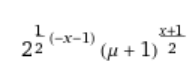
\includegraphics[width=.3\linewidth]{bern1.png}
\caption{entropy of given distribution}
\label{fig:llfunc}
\end{figure}

\section*{Problem 4 (12 pts)}
Consider a binary classification problem in which the target 
values are $t \in  \{0, 1\}$, with a neural 
network output $y(x, w)$ that represents $p(t = 1|x; w)$, and suppose that there is
 a probability $\epsilon$  that the class label on a training data point has been incorrectly set. 
Assuming independent and identically distributed data, write down the error function corresponding to the negative log likelihood. 
What is the error function when $\epsilon=0$? 
Note that this error function makes the model robust to incorrectly labelled data, in contrast to the usual error function.

\subsection*{Your answer here}

The error function can be seen in the figure below with the function when eta=0 below it.
\begin{figure}[h]
\centering
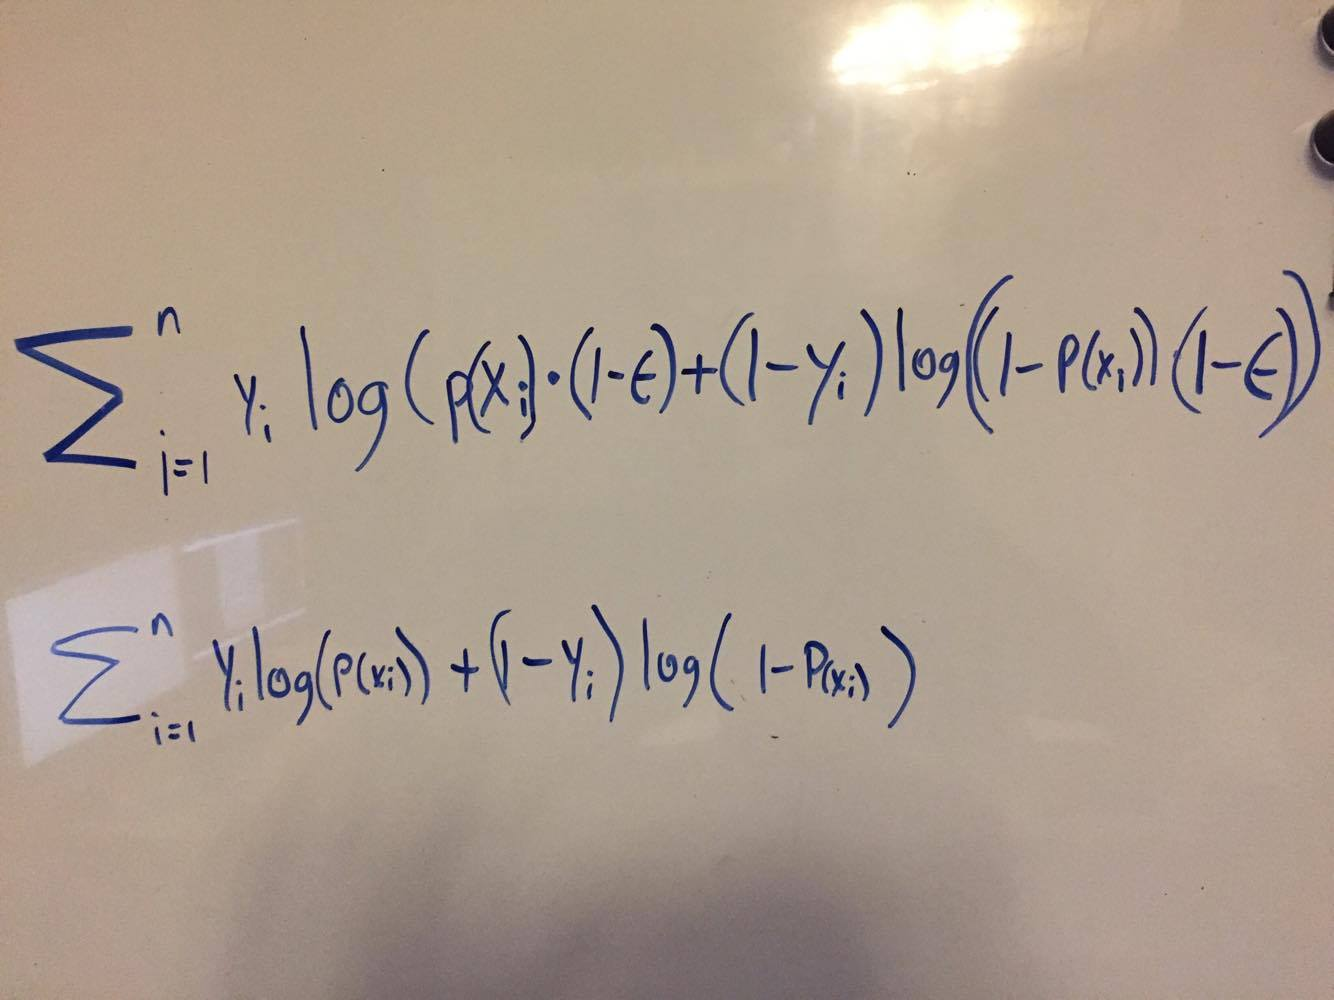
\includegraphics[width=.5\linewidth]{4.jpg}
\caption{negative log likelyhood with uncertainty}
\label{fig:llfunc}
\end{figure}
%Consider the following distribution
%\beqa
%p(x|\sigma,q) = \frac{q}{2(2\sigma^2)^{1/q}\Gamma(1/q)}
%\exp\bigg( - \frac{|x|^q}{2\sigma^2} \bigg)
%\nonumber
%\eeqa
%which is a generalization of the univariate Gaussian distribution. $\Gamma$ is the gamma function.
%\begin{itemize}
%\item (6 pts)
%Show that this distribution
%is normalized so that it represents a valid probability distribution. Also, prove that it reduces to the Gaussian when $q = 2$.
%\item (6 pts) Consider a regression model in which the target variable
%is given by $t = y(x, w) + \epsilon$ where $\epsilon$ is a random noise
%variable drawn from the above distribution and $y(x, w) = w^\top x$. Derive
%the log likelihood function over $w$ and $\sigma^2$, for
%an observed data set of input vectors $X = \{x_1,...,x_N\}$
%and the corresponding target variables $t = (t_1 , . . . , t_N )^{\top}$.
%\end{itemize}

\section*{Problem 5 (8 pts)}
Consider a two-layer network function in which the hidden-unit nonlinear activation functions are given by logistic sigmoid functions of the
form:
\begin{equation}
\sigma(a) = \frac{1}{1 + \exp(-a)}
\end{equation}
Show that there exists an equivalent network, which computes exactly the same 
function, but with hidden unit activation functions 
given by $\tanh(a)$ where the tanh function is defined by:
\begin{equation}
\tanh(a) = \frac{e^a - e^{-a}}{e^a + e^{-a}}
\end{equation}

\subsection*{Your answer here}

The derivation is shown below in the figure below.

\begin{figure}[h]
\centering
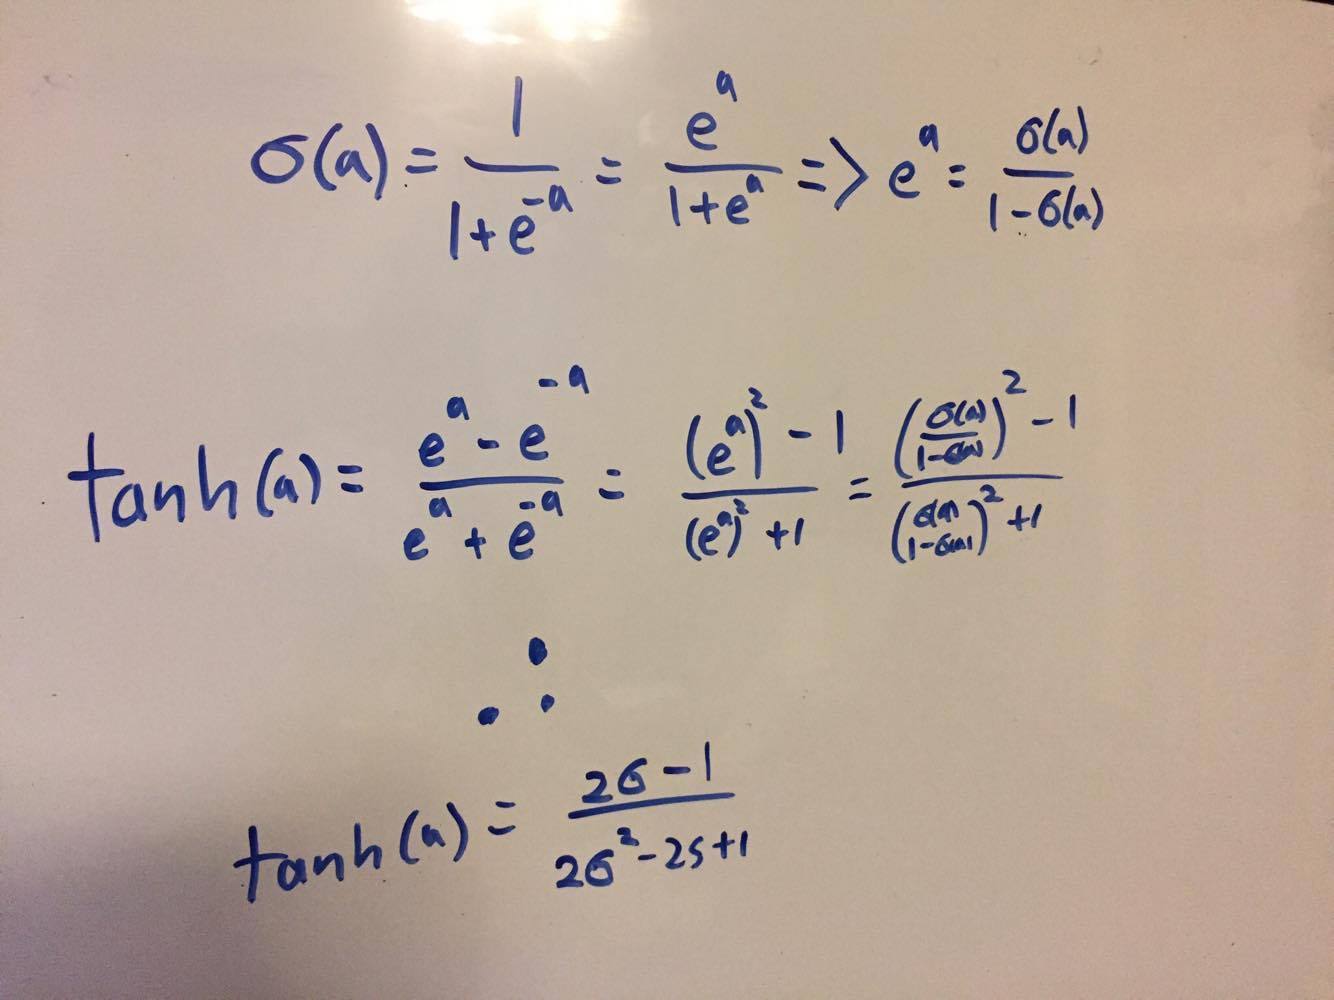
\includegraphics[width=.5\linewidth]{5.jpg}
\caption{derivation of sigmoid into tanh}
\label{fig:sigtan}
\end{figure}


\section*{Problem 6 (60 pts)}

For this question you will 
write your own implementation of backpropagation algorithm for 
training your own neural network.
Please do not use any toolboxes. 
We recommend that you use MATLAB or Python, but you are welcome
to use any other programming language if you wish. 
\\
 
The goal is to label images of
10 handwritten digits of ``zero'', ``one'',..., ``nine''.
The images are 28 by 28 in size (MNIST dataset), which we will be represented
as a vector $x$ of dimension 784 by listing all the pixel values in
raster scan order. The labels t are 0,1,2,...,9 corresponding to
10 classes as written in the image.
There are 3000 training cases, containing 300 examples of each of 10 
classes, 
1000 validation (100 examples of each of 10 classes), and 3000 
test cases (300 examples of each of 10 classes). 
they can be found in the file digitstrain.txt, digitsvalid.txt
 and digitstest.txt: \\
http://www.cs.cmu.edu/$\sim$rsalakhu/10707/assignments.html
\\

{\bf Format of the data}: digitstrain.txt contains 3000 lines.
Each line contains 785 numbers (comma delimited): 
the first 784 real-valued numbers
correspond to the
784 pixel values, and the last number denotes
the class label: 0 corresponds to digit 0, 1 corresponds to digit 1, etc. 
digitsvalid.txt and digitstest.txt contain 1000 and 3000 lines 
and use the same format as above.
As a warm up question, load the data and plot a few examples. Decide if the pixels were scanned out in row-major or column-major order.



\subsubsection*{Backpropagation Algorithm}
Implement backpropagation algorithm with sigmoid activation function 
in a single-layer neural network. The output layer should be 
a softmax output over 10 classes
corresponding to 10 classes of handwritten digits. 
Your backprop code should minimize the cross-entropy entropy function 
for multi-class classification problem.
 

\subsubsection*{a) Basic generalization [5 points]}
Train a single layer neural network with 100 hidden units
(with architecture: 784 $\rightarrow$ 100 $\rightarrow$  10).  
You should
use initialization scheme discussed in class as well as choose a reasonable 
learning rate (e.g. 0.1). Train the network 
repeatedly (more than 5 times) using different random seeds, 
so that each time, you start with a slightly different initialization of 
the weights. 
Run the optimization for at least 200 epochs each time.
If you observe underfitting, continue training the network
for more epochs until you start seeing overfitting.
\\
  
Plot the average training cross-entropy error (sum of 
the cross-entropy error terms over the training dataset  divided by the total number 
of training example) on the y-axis vs. the epoch number (x-axis). 
On the same figure, plot the average validation cross-entropy error function.
\\
 
Examine the plots of training error and validation error (generalization).
How does the network's performance differ on the training set versus the validation set
during learning? Use the plot of error curves (training and validation) to support your argument.



\subsection*{Your answer here}

As you can see in Figure ~\ref{fig:6a},the performance of both the test set and the validation set start out fairly equal. This is the case with both measures of performance, cross-entropy loss and prediction accuracy. 

Soon, however, the model begins to fit better to the training set than the validation set. While the validation set performance still improves, the improvement of train set data is faster.

Eventually, convergence is reached and performance of the validation set stays the same while the performance of the train set marginally increases over time.

When comparing cross entropy error with classification error, the charts seem very similar. The only observable difference is that the cross entropy loss seems to be more similar than the prediction accuracy. This could be because similar numerals were almost predicted correctly in validation set, but lost out to different class.


\begin{figure}
\centering
\begin{subfigure}{.5\textwidth}
  \centering
  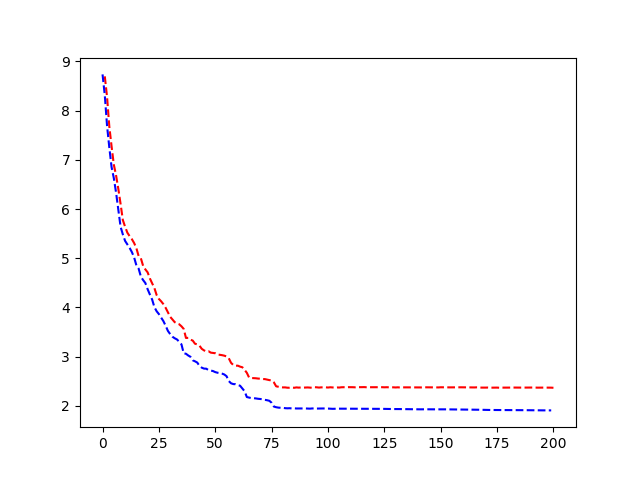
\includegraphics[width=.8\linewidth]{q6a.png}
  \caption{Cross Entropy Error}
  \label{fig:sub1}
\end{subfigure}%
\begin{subfigure}{.5\textwidth}
  \centering
  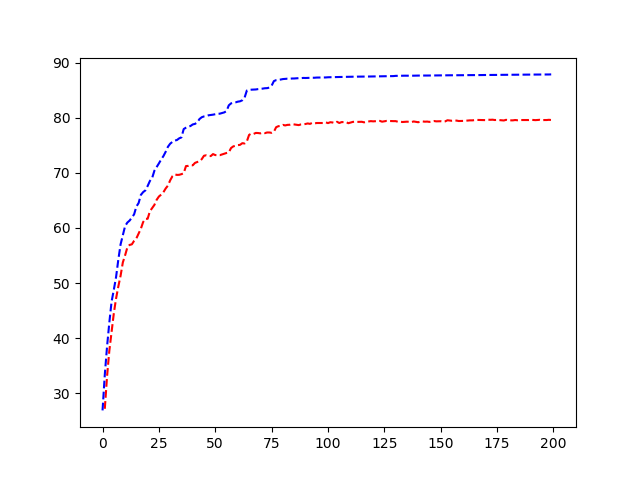
\includegraphics[width=.8\linewidth]{q6b.png}
  \caption{Prediction Accuracy}
  \label{fig:sub2}
\end{subfigure}
\caption{A comparison of two error measures on validation and train data}
\label{fig:6a}
\end{figure}



\subsubsection*{b) Classification error [5 points]}

You should implement an alternative performance measure to the cross entropy, the mean
classification error. You can
consider the output correct if the correct label is given a higher probability
than the incorrect label. You should then count up the total number of
examples that are classified incorrectly (divided by the total number of examples) 
according to this criterion for
training and validation respectively, and maintain this statistic at the end of
each epoch. Plot the classification error (in percentage)  vs. number of epochs, for both
training and validation.
Do you observe a different behavior compared to the behavior of the cross-entropy 
error function? 

\subsection*{Your answer here}
Question answered in section A.

\subsubsection*{c) Visualizing Parameters [5 points]}
Visualize your best results of the learned W as 100 28x28 images 
(plot all filters as one image, as we have seen in class). 
Do the learned features exhibit any structure?

\subsection*{Your answer here}

\begin{figure}[h]
\centering
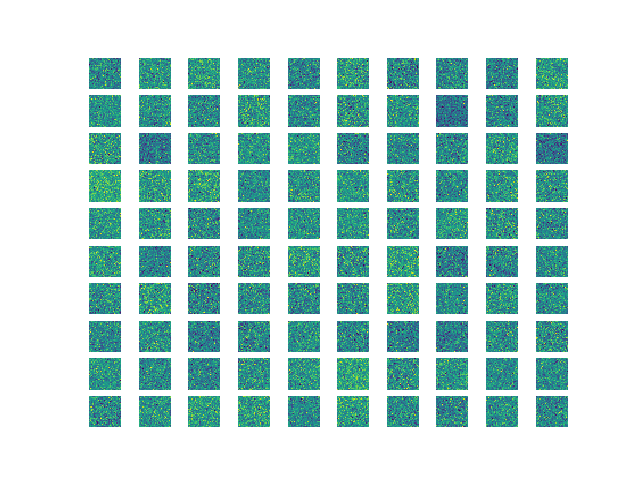
\includegraphics[width=.7\linewidth]{q6c.png}
\caption{sample of hidden layer weights}
\label{fig:weights}
\end{figure}

While at first glance, the weights in Figure ~\ref{fig:weights} may appear to be noisy, one can see structure taking the shape of streaks at different angles and intercepts. 
While we were told to use at least 200 epochs, my network seems to have completely fit in 75. For this reason, I believe that the weights would appear more structured if they were taken from this moment. As epochs went on, overfitting may have caused weights to pick up on less general details about the training set.

\subsubsection*{d) Learning rate [5 points]}
Try different values of the learning rate $\epsilon$. 
You should start with a learning rate of 0.1. 
You should then reduce it to $.01$, and increase it to $0.2$ and
$0.5$. What happens to the convergence properties of the algorithm (looking at
both average cross entropy and \% Incorrect)? Try momentum of $\{0.0, 0.5, 0.9\}$. How does
momentum affect convergence rate? How would you choose the best value of these
parameters?

\subsection*{Your answer here}

As you can see in Figure ~\ref{fig:eta}, the learning rate had an extremely large effect on convergence. Namely, the higher the learning rate, the faster the network converged.

\begin{figure}[h]
\centering
\begin{subfigure}{.5\textwidth}
  \centering
  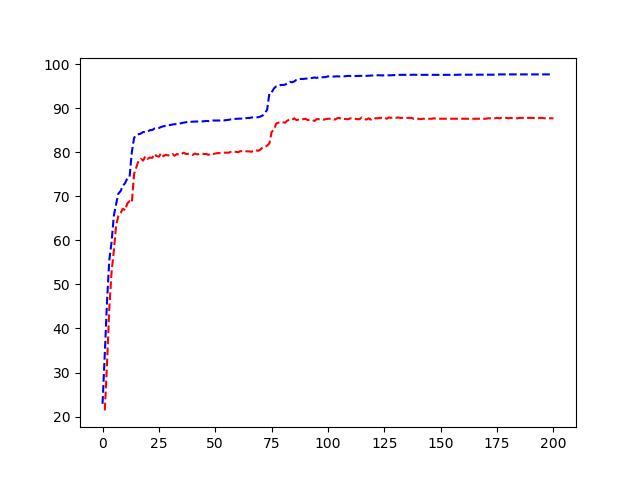
\includegraphics[width=.8\linewidth]{eta01ac.png}
  \caption{eta = 0.1}
  \label{fig:sub1}
\end{subfigure}%
\begin{subfigure}{.5\textwidth}
  \centering
  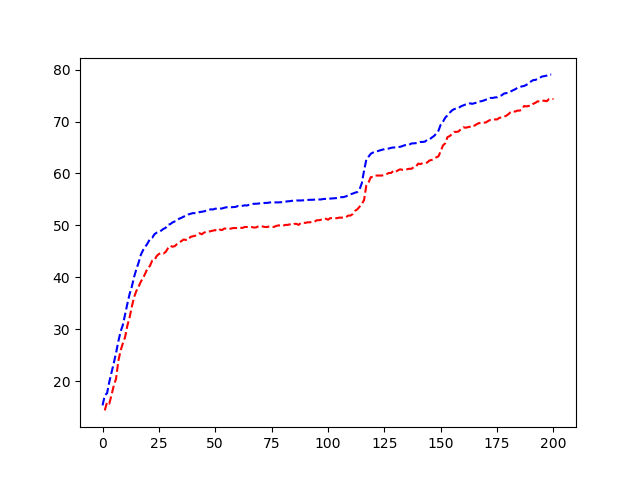
\includegraphics[width=.8\linewidth]{eta001ac.png}
  \caption{eta = 0.01}
  \label{fig:sub2}
\end{subfigure}
\caption{a comparison of the conversion of different learning rates}
\label{fig:eta}
\end{figure}
 When factoring in momentum, the effects were less clear. However momentum did seem to improve the convergence rate overall. Show in Figure \ref{fig:momentum}, are some interesting effects caused when the momentum rate was 0.5. The network's accuracy seemed to plateau and then jump up multiple times.

\begin{figure}[h]
\centering
\begin{subfigure}{.5\textwidth}
  \centering
  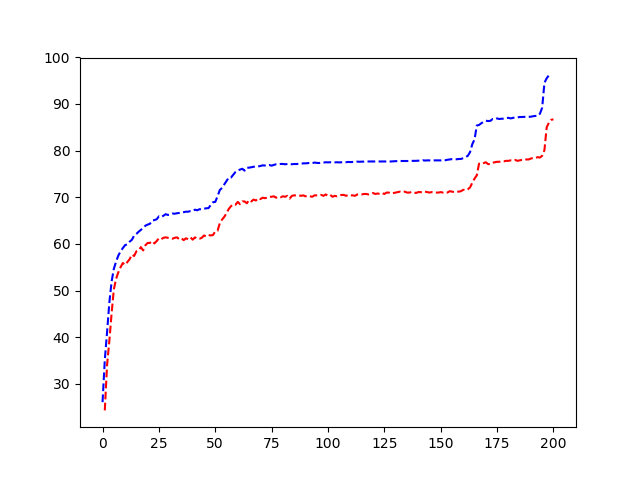
\includegraphics[width=.8\linewidth]{m5ac.png}
  \caption{momentum = 0.5}
  \label{fig:sub1}
\end{subfigure}%
\begin{subfigure}{.5\textwidth}
  \centering
  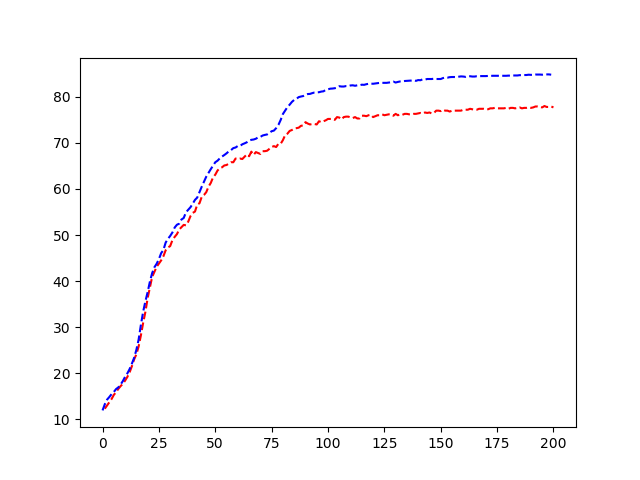
\includegraphics[width=.8\linewidth]{m9ac.png}
  \caption{momentum = 0.9}
  \label{fig:sub2}
\end{subfigure}
\caption{a comparison of the conversion of different momentum rates}
\label{fig:momentum}
\end{figure}

\subsubsection*{e) Number of hidden units [5 points]}
Set the learning rate $\epsilon$ to $.01$, momentum to $0.5$ and try different numbers of
hidden units on this problem.
You should try training a network with 20, 100, 200, and 500  hidden units.
Describe the effect of this modification on the convergence properties, and the
generalization of the network.

To find the best parameters, I would use choose a range of each one which I thought was reasonable and perform either a random search or a grid search on these parameters.

\subsection*{Your answer here}
As the number of units increased, performance actually seemed to decrease in the network. That said, even though convergence was slowed, the actual generalization of the network seemed to be improved. Figure \ref{fig:hu} shows these effects.

\begin{figure}[h]
\centering
\begin{subfigure}{.5\textwidth}
  \centering
  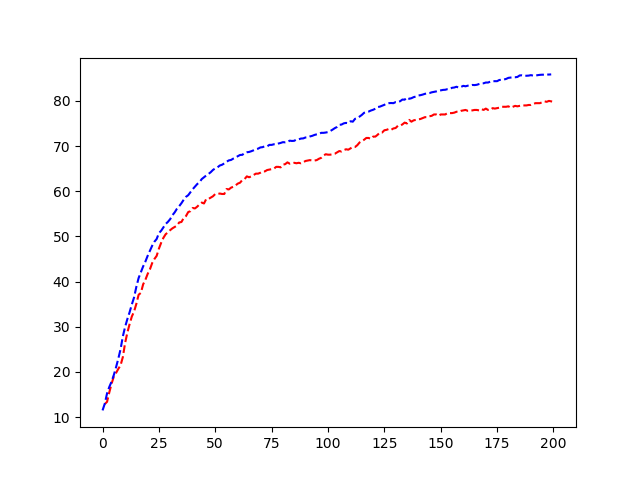
\includegraphics[width=.8\linewidth]{20huac.png}
  \caption{20 hidden units}
  \label{fig:sub1}
\end{subfigure}%
\begin{subfigure}{.5\textwidth}
  \centering
  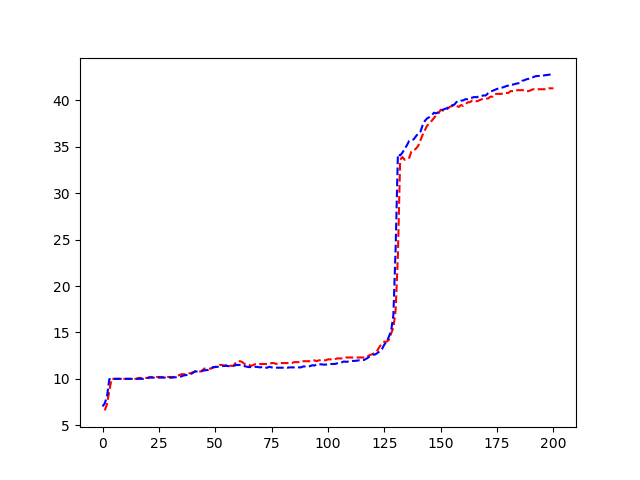
\includegraphics[width=.8\linewidth]{500huac.png}
  \caption{500 hidden units}
  \label{fig:sub2}
\end{subfigure}
\caption{a comparison of the accuracy of numbers of hidden units}
\label{fig:hu}
\end{figure}

\subsubsection*{f) Best performing single-layer network [10 points]}
Cross-validation: 
Explore various model hyper-parameters, including 
\begin{itemize}
\item learning rates
\vspace{-0.09in}
\item momentum
\vspace{-0.09in}
\item number of hidden units in each layer
\vspace{-0.09in}
\item number of epochs (early stopping)
\vspace{-0.09in}
\item $L_2$ regularization (weight decay)
\end{itemize}
to achieve the best validation accuracy. Briefly describe your findings.
\\

Given the best found values, report the final performance of your 1-layer neural
network (both average cross entropy and \% Incorrect) on the training, validation, and test sets.
Visualize your best results of the learned W as 28x28 images 
(plot all filters as one image, as we have seen in class).

\subsection*{Your answer here}
I found that the best learning rates tended to be higher, my best one was eta=0.5. Because I was using a high learning rate, I also employed early stopping and only ran for 18 epochs. I did not use momentum as it caused worse performance. I ended up sticking with 100 hidden units, as this had the best performance once the other hyperparameters were set. L2 regularization did help and was used.
Statistics for each set of data:
Train:
Accuracy = 97.1
Cross Entropy = 0.28
Validation:
Accuracy = 88.9
Cross Entropy = 0.60
Test:
Accuracy = 87.46
Cross Entropy = 0.71
Figure ~\ref{fig:weights2} shows the vizualization of the weights for this network.

\begin{figure}[h]
\centering
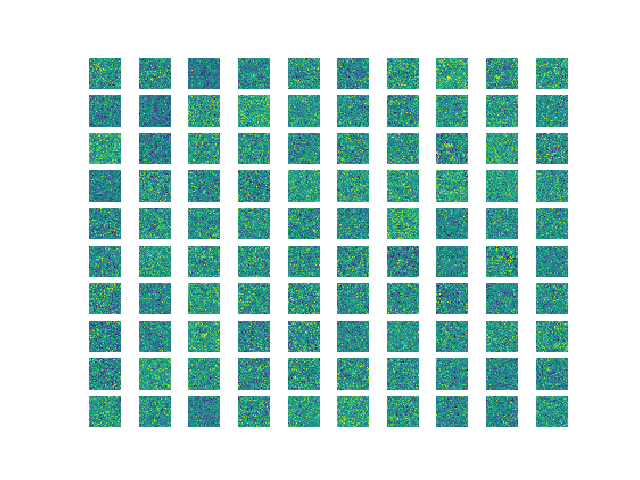
\includegraphics[width=.7\linewidth]{q6f_weights.png}
\caption{sample of hidden layer weights}
\label{fig:weights2}
\end{figure}

\subsubsection*{g) Extension to multiple layers [10 points]}
Implement a 2-layer neural network, starting with a simple architecture 
containing 100 hidden units in each layer
(with architecture: 784 $\rightarrow$ 100 $\rightarrow$ 100 $\rightarrow$  10).
\\
  
Cross-validation: Explore various model hyper-parameters, including learning rates, 
momentum, number of hidden units in each layer, number of epochs, and weight decay 
to achieve the best validation accuracy. Briefly describe your findings.  
\\

Given the best found values, report the final performance of your 2-layer neural
network (both average cross entropy and \% Incorrect) on the training, validation, and test sets.
Visualize your best results of the learned 1st-layer W as 28x28 images 
(plot all filters as one image, as we have seen in class).
How do these filters compare to the ones you obtained when training a
single-layer network?
\\

Does 1-layer network outperform a 2-layer model in term of generalization capabilities?


\subsection*{Your answer here}

While I believe that a 2-layer model should be able to outperform, I could not find hyperparameters that recieved better performance.

I found that I was able to train for many more epochs before plateauing of the validation accuracy, however I also found that it was much easier to overfit on the training data.
Learning rate = .03
Epochs = 500
Momentum = 0.9
Layers = [10,20]


Statistics for each set of data:
Train:
Accuracy = 90.5
Cross Entropy = 0.46
Validation:
Accuracy = 82.2
Cross Entropy = 0.67
Test:
Accuracy = 78.9
Cross Entropy = 0.75

Figure ~\ref{fig:weights3} shows the weights of my first layer. The structure in these weights appears to be more complicated than the previous ones. Rather than simple lines at different angles, the weights show structures such as loops and curves. This may be because there were much fewer weights in my first layer.

\begin{figure}
\centering
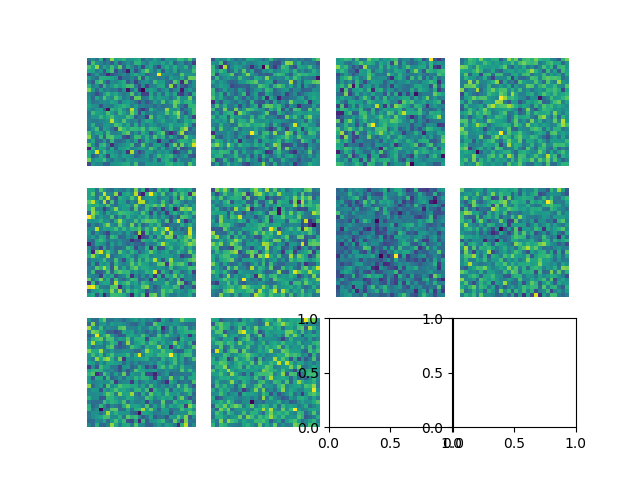
\includegraphics[width=.7\linewidth]{gweights.png}
\caption{sample of hidden layer weights}
\label{fig:weights3}
\end{figure}

\subsubsection*{h) Batch Normalization [10 points]}

For your two-layer network, implement batch normalization for a batch size of 32. Describe how batch norm helps (or doesn't help) in terms of speed and accuracy (train and validation). 


\subsection*{Your answer here}
Batch normalization did not necessarily help with speed to convergence, however I did find that it helped the network with accuracy. The generalization of the network was also improved, as the loss difference between the train and validation sets were smaller.

\subsubsection*{i) Different Activation Functions [5 points]}

Now, change the activation functions to ReLU and tanh instead of the original sigmoid. Do you see any difference in terms of performance or accuracy ? Report your findings.

\subsection*{Your answer here}

ReLU seemed to perform marginally better in all aspects, however there were different optimal hyperparameters.

TanH performed horribly, and I could not find a set of hyperparameters that worked.



\end{document}


